\documentclass[12pt]{article}
\usepackage[paperwidth=36in,paperheight=24in,margin=0in]{geometry}
\usepackage{tikz}
\usetikzlibrary{calc,arrows.meta,positioning,shapes.geometric}
\usepackage{xcolor,graphicx,amsmath,amssymb,array,booktabs,ragged2e}
\usepackage{librebaskerville}
\usepackage[defaultfam,tabular,lining]{montserrat}
\usepackage[T1]{fontenc}
\usepackage{hyperref}
\pagestyle{empty}
\setlength{\parindent}{0pt}
\setlength{\parskip}{0pt}

\definecolor{navy}{HTML}{235078}
\definecolor{teal}{HTML}{1482A5}
\definecolor{leafgreen}{HTML}{8CD23C}
\definecolor{bodytext}{HTML}{333333}
\definecolor{softblue}{HTML}{EAF7FA}
\definecolor{linegray}{HTML}{A8B3B8}
\definecolor{orange}{HTML}{D45B0A}
\definecolor{card}{HTML}{FFFFFF}
\hypersetup{colorlinks=true,urlcolor=navy,linkcolor=navy}

% ---------- TEMPLATE BACKGROUND ----------
\newcommand{\bg}{%
  \fill[white] (origin) rectangle ([xshift=36in,yshift=-24in]origin);
  \fill[softblue] ([yshift=-4.88in]origin) rectangle ([xshift=36in,yshift=-24in]origin);
  \draw[navy,line width=0.42in]
    (origin) ++(0,-5.03in)
    .. controls +(6in,0.38in) and +(-5in,0.38in) .. ++(18in,0)
    .. controls +(6in,-0.10in) and +(-5in,0.24in) .. ++(18in,-0.16in);
  \draw[leafgreen,line width=0.10in]
    (origin) ++(0,-5.02in)
    .. controls +(7in,0.40in) and +(-5in,0.45in) .. ++(18in,0.01in)
    .. controls +(6in,-0.12in) and +(-5in,0.22in) .. ++(18in,-0.14in);
  \fill[leafgreen] ([yshift=0.48in]current page.south west) rectangle ([yshift=0.62in]current page.south east);
  \fill[navy] ([yshift=0.16in]current page.south west) rectangle ([yshift=0.48in]current page.south east);
}

\newcommand{\logo}{%
  % The supplied PNGs occupy the former logo-box footprints exactly.
  % No navy rectangle is drawn behind them; the surrounding poster background is white.
  \node[anchor=north west,inner sep=0pt] at ([xshift=1.34in,yshift=-1.14in]current page.north west)
    {
\includegraphics[width=2.74in,height=2.43in]{assets/logo_left.png}};
  \node[anchor=north west,inner sep=0pt] at ([xshift=31.92in,yshift=-1.15in]current page.north west)
    {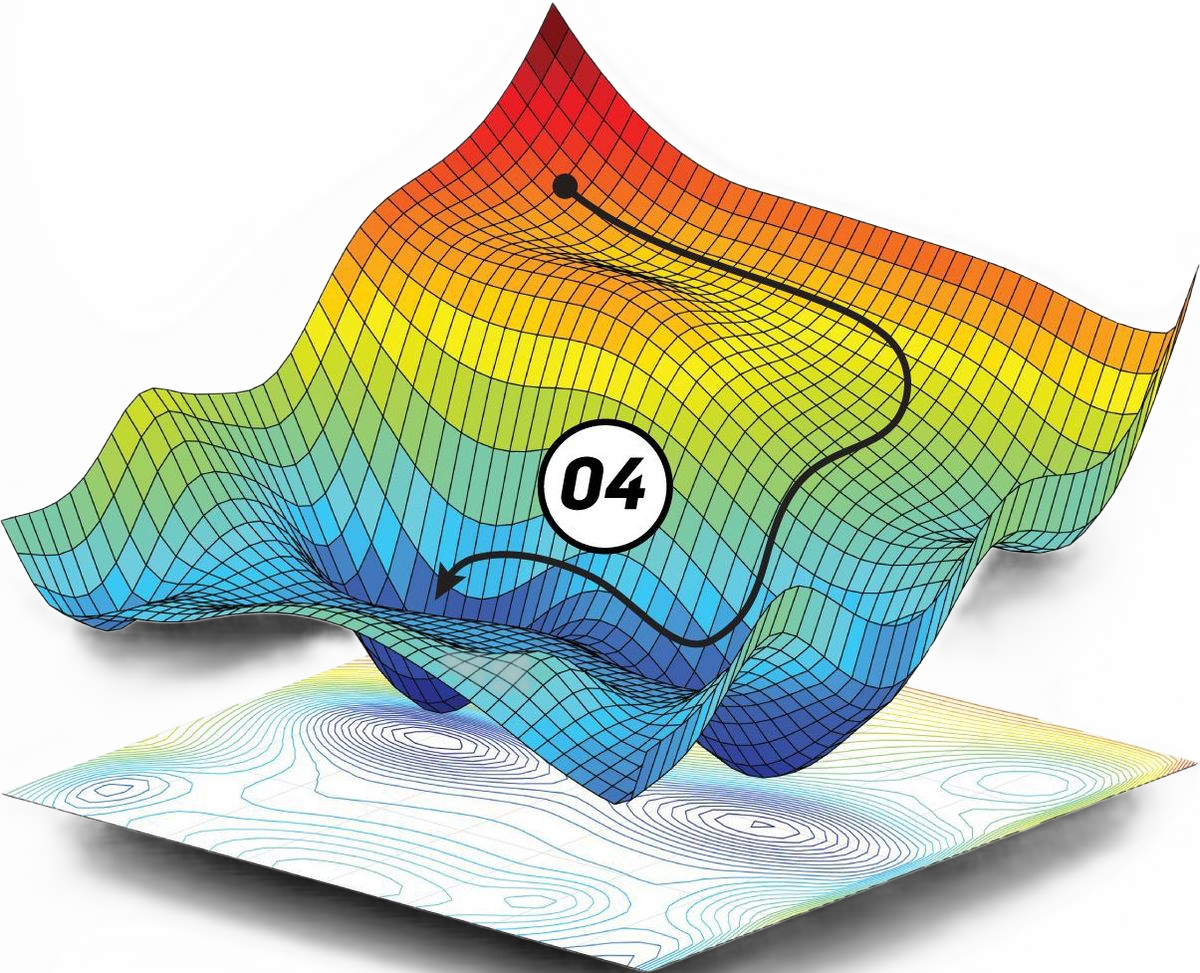
\includegraphics[width=2.75in,height=2.43in]{assets/logo_right.png}};
}

\newcommand{\header}[2]{%
  \node[anchor=center,align=center,text width=27in,
        font=\rmfamily\fontsize{68}{75}\selectfont,text=navy]
    at ([xshift=18in,yshift=-1.48in]current page.north west) {#1};
  \node[anchor=center,align=center,text width=27in,
        font=\sffamily\fontsize{24}{29}\selectfont,text=navy]
    at ([xshift=18in,yshift=-2.72in]current page.north west) {#2};
}

\newcommand{\footer}{%
  \fill[navy] ([yshift=0.16in]current page.south west) rectangle ([yshift=0.48in]current page.south east);
  \fill[leafgreen] ([yshift=0.48in]current page.south west) rectangle ([yshift=0.53in]current page.south east);
  \node[anchor=west,font=\sffamily\fontsize{11}{13}\selectfont,text=white]
    at ([xshift=1.30in,yshift=0.32in]current page.south west) {Poster Presentation};
  \node[anchor=center,font=\sffamily\fontsize{11}{13}\selectfont,text=white]
    at ([xshift=18in,yshift=0.32in]current page.south west) {Advanced Algorithms (CSE 375)};
  \node[anchor=east,align=right,font=\sffamily\fontsize{10.2}{12}\selectfont,text=white]
    at ([xshift=-1.15in,yshift=0.32in]current page.south east)
    {2023100000230@seu.edu.bd\quad 2022200000179@seu.edu.bd};
}

\newcommand{\sectionbar}[5]{%
  \fill[teal] ([xshift=#1in,yshift=-#2in]current page.north west)
    rectangle ([xshift=#1in+#3in,yshift=-#2in-#4in]current page.north west);
  \node[anchor=center,align=center,text width=#3in,
        font=\rmfamily\bfseries\fontsize{24}{28}\selectfont,text=white]
    at ([xshift=#1in+0.5*#3in,yshift=-#2in-0.5*#4in]current page.north west) {#5};
}

% The text area is intentionally narrower than the card so nothing can cross the border.
\newcommand{\card}[5]{%
  \fill[card] ([xshift=#1in,yshift=-#2in]current page.north west)
    rectangle ([xshift=#1in+#3in,yshift=-#2in-#4in]current page.north west);
  \draw[linegray,line width=0.8pt] ([xshift=#1in,yshift=-#2in]current page.north west)
    rectangle ([xshift=#1in+#3in,yshift=-#2in-#4in]current page.north west);
  \node[anchor=north west,inner sep=0pt,outer sep=0pt]
    at ([xshift=#1in+0.22in,yshift=-#2in-0.20in]current page.north west) {\begin{minipage}[t]{\dimexpr #3in-0.44in\relax}#5\end{minipage}};
}

\newcommand{\body}{\sffamily\fontsize{20}{24}\selectfont\color{bodytext}\RaggedRight}
\newcommand{\bodycompact}{\sffamily\fontsize{18.6}{22.3}\selectfont\color{bodytext}\RaggedRight}
\newcommand{\introtext}{\sffamily\fontsize{17.2}{20.2}\selectfont\color{bodytext}\RaggedRight}
\newcommand{\titlein}{\rmfamily\bfseries\fontsize{21}{25}\selectfont\color{orange}}
\newcommand{\captiontext}{\sffamily\bfseries\fontsize{14.2}{17}\selectfont\color{navy}}
\newcommand{\eq}{\begin{center}\displaystyle\fontsize{25}{30}\selectfont}

\begin{document}

% =============================================================
% PAGE 1
% =============================================================
\begin{tikzpicture}[remember picture,overlay]
\coordinate (origin) at (current page.north west);
\path[use as bounding box] (0,0) rectangle (36in,-24in);
\bg\logo
\header{Gradient Descent}{Ruhid Ghosh (ID: 2023100000230)\\[-1pt]Sadia Alam (ID: 2022200000179)\\[-1pt]Southeast University}

% ---------------- TOP ROW ----------------
\sectionbar{0.58}{5.72}{8.10}{0.66}{Introduction}
\card{0.58}{6.50}{8.10}{8.65}{%
\introtext
\textbf{Gradient Descent} is an optimization algorithm used to minimize a function, usually a cost function in machine learning or deep learning.\\[5pt]
\textbf{Key Application:} Sales Prediction, Linear Regression, Neural Networks.\\[6pt]
\textbf{Problem Statement \& The Initial Approach:} A company wants to predict its sales based on advertising expenditure. However, the initial model produces inaccurate predictions because its parameters (weights) are not optimized. Therefore, an optimization method is needed to iteratively adjust the model parameters and minimize the prediction error.\\[6pt]
\textbf{Key Idea:} Iterative weight optimization.\\[2pt]
\textbf{Improving Accuracy:} Learning Rate \& Iterative Updates.\\[5pt]
{\titlein The Gradient Descent Algorithm base\par}\vspace{4pt}
Gradient Descent is based on moving in the opposite direction of the gradient to minimize the loss function. The gradient indicates the direction of the steepest increase in loss. Therefore, moving in the opposite direction reduces the loss.\\[6pt]
\textbf{Loss Function (MSE):}
\[
J(w)=\frac{1}{m}\sum_{i=1}^{m}\left(h(x_i)-y_i\right)^2
\]
\textbf{Here:} $J(w)$ = cost/loss function; $m$ = total training examples; $h(x_i)$ = model prediction; $h(x_i)-y_i$ = prediction error.
\\[6pt]
\textbf{Weight Update Rule:}
\[
w_{new}=w_{old}-\alpha\frac{\partial J(w)}{\partial w}
\]
}

\sectionbar{8.93}{5.72}{18.00}{0.66}{Gradient Descent Visualization}
\card{8.93}{6.50}{18.00}{8.05}{%
\bodycompact
The gradient indicates the direction of the steepest increase in loss. Gradient Descent moves in the opposite direction and repeatedly updates the parameters until the loss is minimized.\\[7pt]
\begin{center}
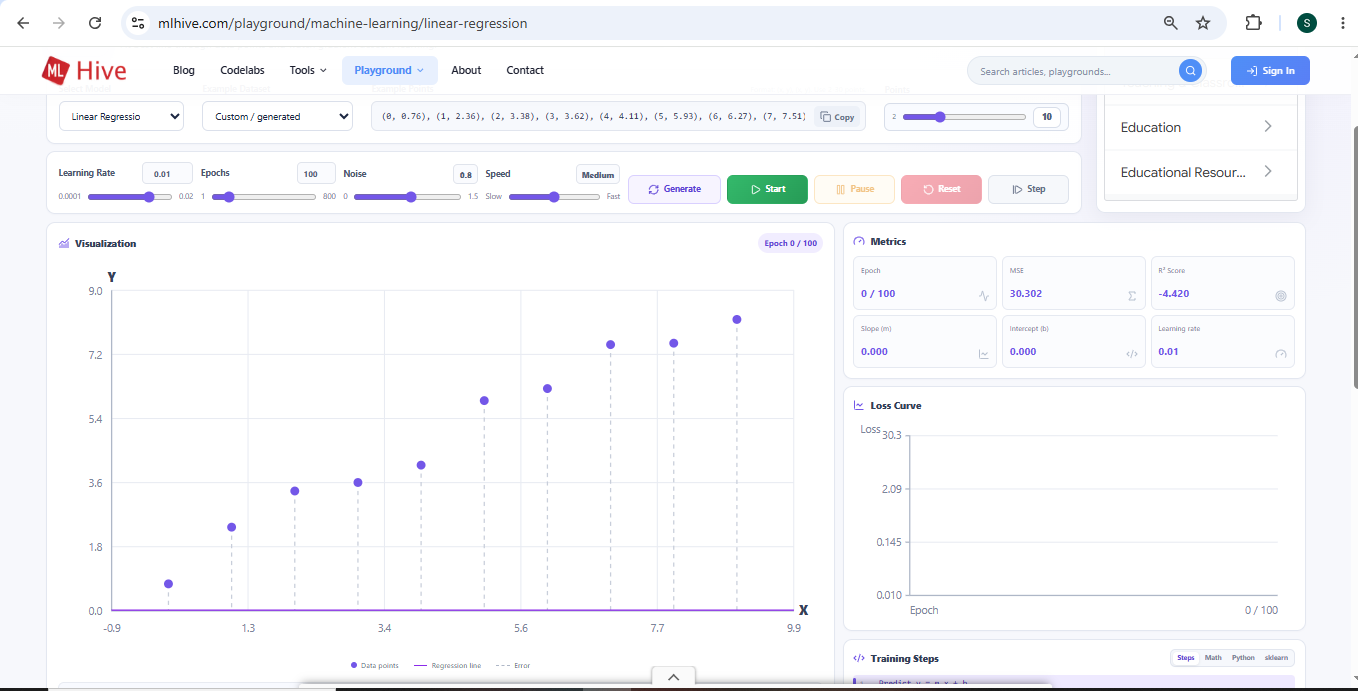
\includegraphics[width=7.9in,height=3.75in,keepaspectratio]{assets/p3_1.png}\hspace{0.35in}
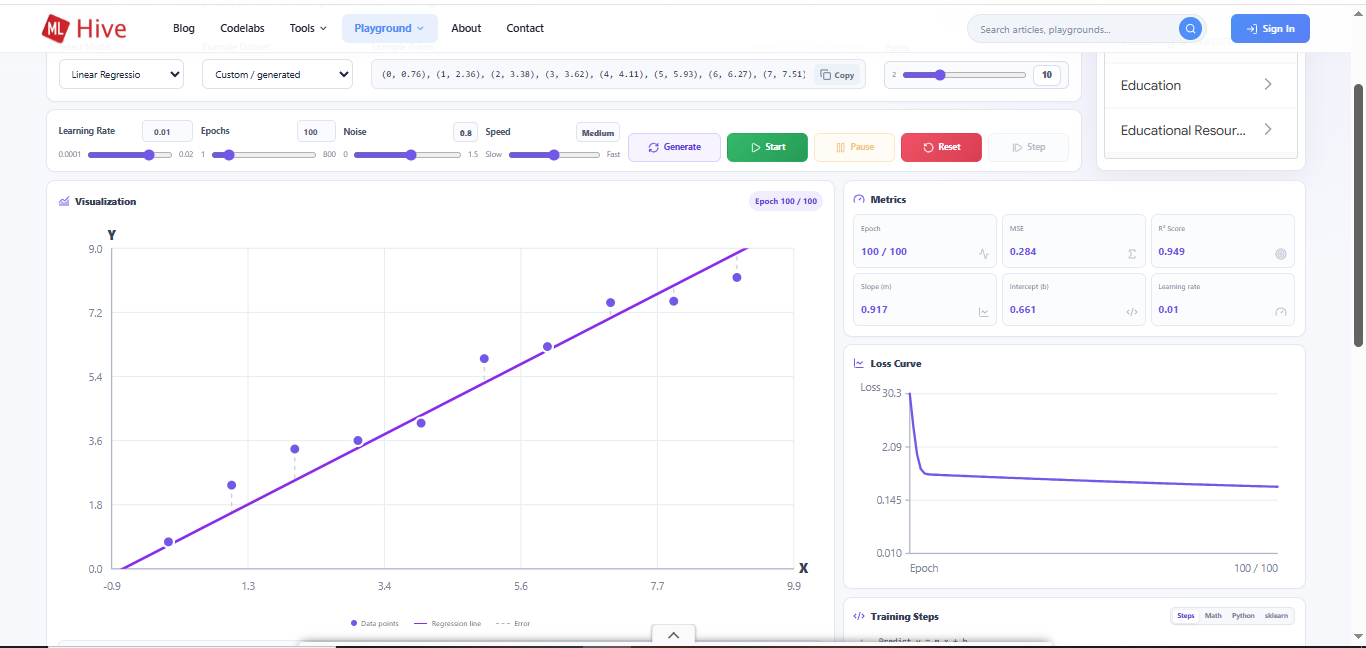
\includegraphics[width=7.9in,height=3.75in,keepaspectratio]{assets/p3_2.png}
\end{center}
\vspace{2pt}
\begin{minipage}[t]{7.85in}\centering\captiontext Initial State — Before Optimization\end{minipage}
\hfill
\begin{minipage}[t]{7.85in}\centering\captiontext Optimized State — After Gradient Descent\end{minipage}
\\[8pt]
\begin{center}
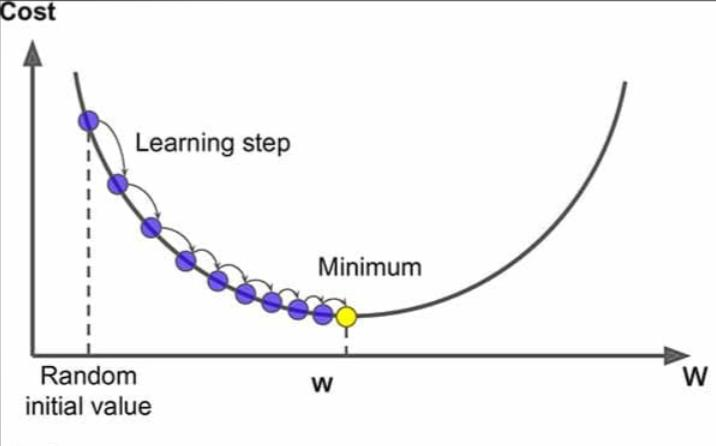
\includegraphics[width=5.7in,height=1.55in,keepaspectratio]{assets/p2_1.jpeg}
\end{center}
\vspace{1pt}
\begin{center}\sffamily\fontsize{13.5}{16}\selectfont\color{navy}
\textbf{Reference:}\; \href{https://www.mlhive.com/playground/machine-learning/linear-regression}{Linear Regression Visualizer - ML Hive Playground}
\end{center}
}

\sectionbar{27.28}{5.72}{8.14}{0.66}{Algorithmic Execution Process}
\card{27.28}{6.50}{8.14}{8.05}{%
\bodycompact
\textbf{Step 1: Initialize Parameters} — Set initial weights $w$, bias $b$, and learning rate $\alpha$.\\[5pt]
\textbf{Step 2: Make Prediction} — Calculate $h(x)=wx+b$.\\[5pt]
\textbf{Step 3: Calculate Loss} — Measure the prediction error using the Cost/Loss Function.
\[
J(w)=\frac{1}{m}\sum_{i=1}^{m}(h(x_i)-y_i)^2
\]
\textbf{Step 4: Compute Gradient} — Calculate the gradient of the loss with respect to the weight:
\[
\frac{\partial J(w)}{\partial w}
\]
\textbf{Step 5: Update Parameters} — Adjust the weight to reduce the loss:
\[
w_{new}=w_{old}-\alpha\frac{\partial J(w)}{\partial w}
\]
\textbf{Step 6: Repeat Until Convergence} — Repeat prediction, loss calculation, gradient computation, and parameter update until the loss is minimized.
}

% ---------------- BOTTOM ROW ----------------
\sectionbar{0.58}{15.35}{8.10}{0.66}{Graph Shows}
\card{0.58}{16.13}{8.10}{6.50}{%
\bodycompact
\begin{center}
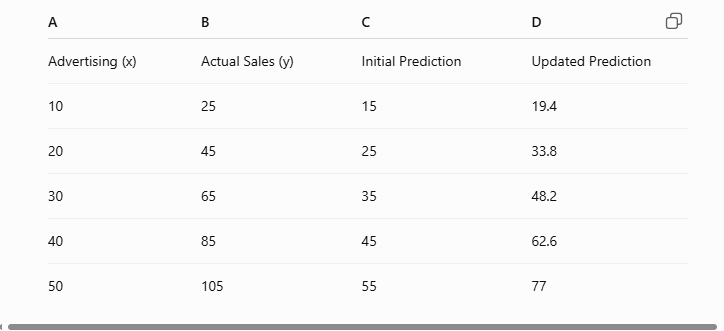
\includegraphics[width=3.25in,height=2.45in,keepaspectratio]{assets/p4_1.png}\hspace{0.18in}
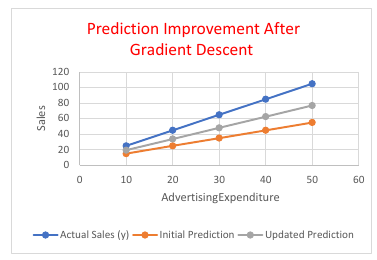
\includegraphics[width=3.25in,height=2.45in,keepaspectratio]{assets/p4_prediction_chart.png}
\end{center}
\vspace{2pt}
\textbf{Graph Shows}\\[2pt]
As advertising expenditure increases, sales also increase. Initially, the model's predictions are far from the actual sales values. After the Gradient Descent weight update, the prediction line moves closer to the actual sales points. This reduces prediction error (loss) and improves model accuracy.
}

\sectionbar{8.93}{15.35}{8.14}{0.66}{Properties of Gradient Descent}
\card{8.93}{16.13}{8.14}{6.50}{%
\bodycompact
\textbullet{} \textbf{Iterative Optimization} — Updates model parameters repeatedly to minimize the loss function.\\[4pt]
\textbullet{} \textbf{Gradient-Based} — Uses the gradient to determine the direction of parameter updates.\\[4pt]
\textbullet{} \textbf{Learning Rate Controlled} — Controls the step size of each update.\\[4pt]
\textbullet{} \textbf{Convergence} — Gradually moves toward a minimum of the loss function.\\[4pt]
\textbullet{} \textbf{Scalable} — Efficiently handles models with a large number of parameters.\\[4pt]
\textbullet{} \textbf{Loss Minimization} — Aims to reduce prediction error and improve model performance.
}

\sectionbar{17.42}{15.35}{9.10}{0.66}{Forward Propagation and Backward Propagation}
\card{17.42}{16.13}{9.10}{6.50}{%
\begin{center}
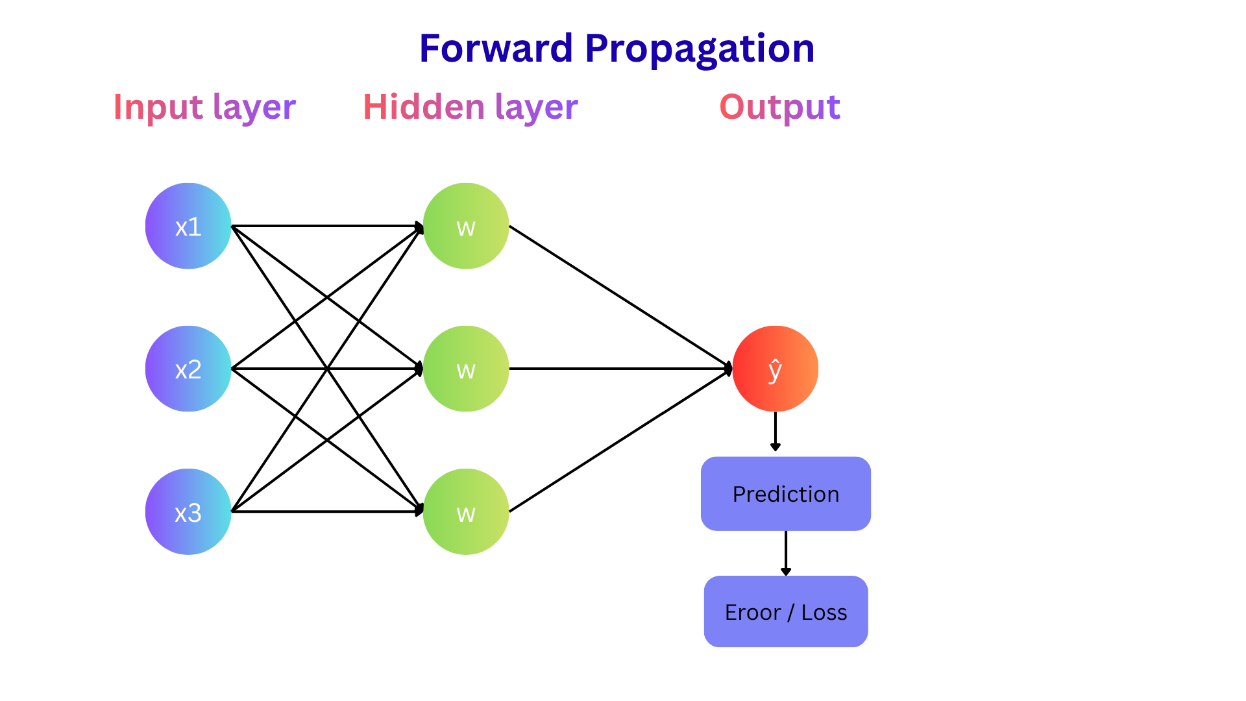
\includegraphics[width=4.05in,height=2.55in,keepaspectratio]{assets/p6_1.png}\hspace{0.15in}
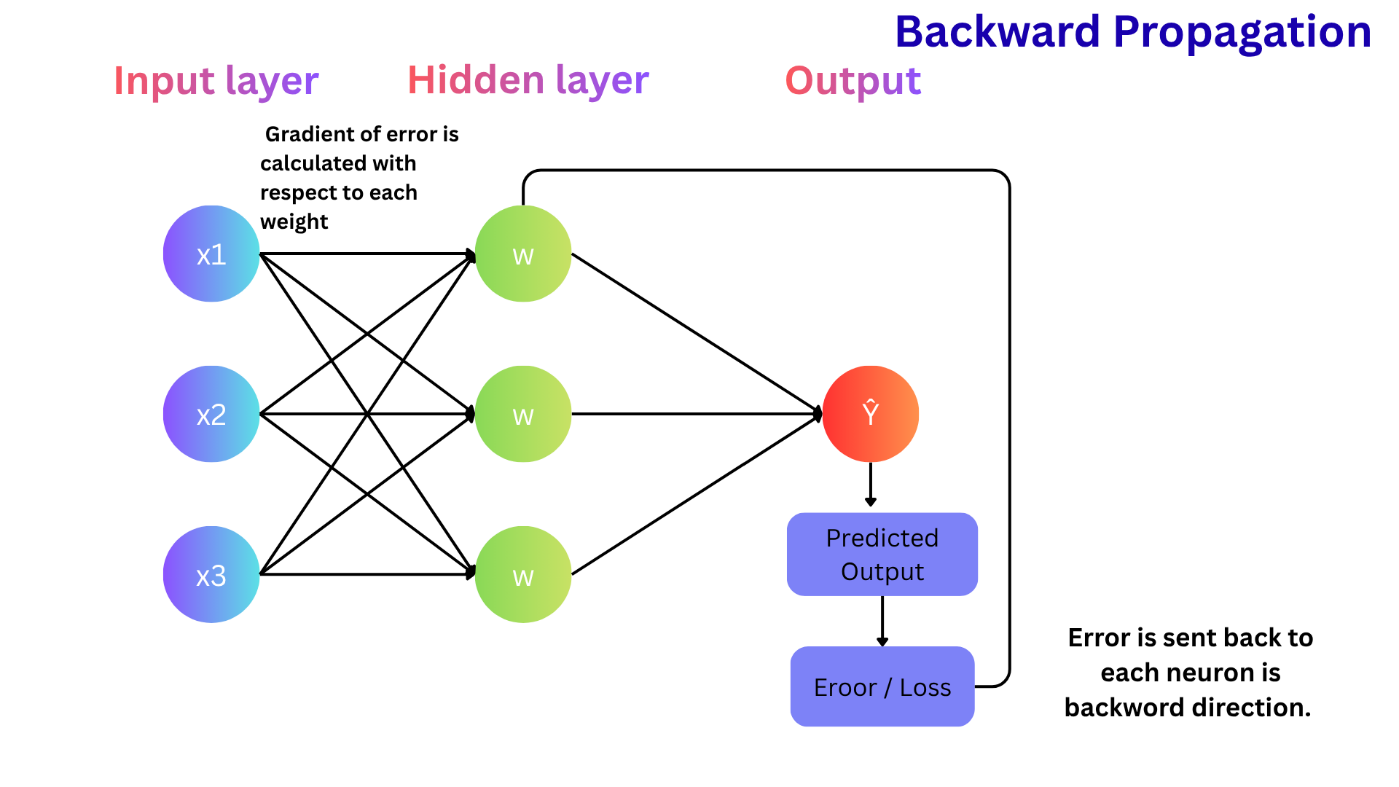
\includegraphics[width=4.05in,height=2.55in,keepaspectratio]{assets/p6_2.png}
\end{center}
\vspace{5pt}
\bodycompact
\textbf{Forward Propagation} passes input data through the network to generate a prediction.\\[7pt]
\textbf{Backward Propagation} propagates the error backward through the network to calculate gradients and adjust the weights for improved predictions.
}

\sectionbar{26.72}{15.35}{8.70}{0.66}{Time and Space Complexity}
\card{26.72}{16.13}{8.70}{6.50}{%
\bodycompact
Let $n$ = number of training samples, $d$ = number of features, and $I$ = number of iterations.\\[6pt]
Each iteration requires approximately $O(n\times d)$ operations to calculate the gradient.\\[7pt]
\textbf{Overall Time Complexity:}
\[
O(I\times n\times d)
\]
\textbf{Space Complexity:} $O(n\times d)$ including training data.\\[6pt]
\textbf{Without training data:} $O(d)$.\\[10pt]
\begin{center}
\fcolorbox{linegray}{softblue}{\parbox{7.25in}{\centering\sffamily\bfseries\fontsize{15.5}{19}\selectfont\color{navy}Gradient Descent reduces the cost function through repeated, gradient-based parameter updates.}}
\end{center}
}

\footer
\end{tikzpicture}
\newpage

% =============================================================
% PAGE 2
% =============================================================
\begin{tikzpicture}[remember picture,overlay]
\coordinate (origin) at (current page.north west);
\path[use as bounding box] (0,0) rectangle (36in,-24in);
\bg\logo
\header{Gradient Descent}{Ruhid Ghosh (ID: 2023100000230)\\[-1pt]Sadia Alam (ID: 2022200000179)\\[-1pt]Southeast University}

% ---------------- TOP ROW ----------------
\sectionbar{0.58}{5.72}{8.25}{0.66}{Stochastic Gradient Descent (SGD)}
\card{0.58}{6.50}{8.25}{8.05}{%
\bodycompact
\textbf{Stochastic Gradient Descent (SGD)} is an optimization algorithm used to minimize a function, usually a cost function in machine learning or deep learning.\\[5pt]
\textbf{Key Application:} Sales Prediction, Linear Regression, Neural Networks.\\[6pt]
\textbf{Problem Statement \& The Initial Approach:} A company wants to predict its sales based on advertising expenditure. However, the initial model produces inaccurate predictions because its parameters (weights) are not optimized. Therefore, an efficient optimization method is needed to iteratively adjust the model parameters and minimize prediction error.\\[6pt]
\textbf{Key Idea:} Iterative weight optimization using individual training examples.\\[2pt]
\textbf{Improving Accuracy:} Learning Rate \& Frequent Weight Updates.\\[7pt]
{\titlein The Stochastic Gradient Descent Algorithm\par}\vspace{4pt}
SGD updates the model weights using one randomly selected training example at a time instead of the entire dataset. For each example, SGD calculates prediction error, computes the gradient, and immediately updates the weight. This makes optimization faster and more frequent, especially for large datasets.
}

\sectionbar{9.10}{5.72}{8.35}{0.66}{Weight Update Rule}
\card{9.10}{6.50}{8.35}{8.05}{%
\bodycompact
\textbf{Loss Function (for one example):}
\[
J_i(w)=\frac{1}{2}\left(h(x_i)-y_i\right)^2
\]
\textbf{Here:} $J_i(w)$ = loss for an individual training sample; $h(x_i)$ = model prediction; $h(x_i)-y_i$ = prediction error.\\[8pt]
\textbf{Weight Update Rule:}
\[
w_{new}=w_{old}-\alpha\frac{\partial J_i(w)}{\partial w}
\]
\textbf{Here:} $\alpha$ = learning rate; $J_i(w)$ = loss for the individual training sample; $\partial J_i(w)/\partial w$ = gradient of the individual loss with respect to the weight.\\[10pt]
\begin{center}
\fcolorbox{linegray}{softblue}{\parbox{6.95in}{\centering\sffamily\bfseries\fontsize{17}{21}\selectfont\color{navy}One example $\rightarrow$ prediction $\rightarrow$ loss $\rightarrow$ gradient $\rightarrow$ immediate weight update}}
\end{center}
}

% Algorithm execution and its properties are intentionally adjacent.
\sectionbar{18.00}{5.72}{8.40}{0.66}{Algorithmic Execution Process — SGD}
\card{18.00}{6.50}{8.40}{8.05}{%
\sffamily\fontsize{15.4}{18.2}\selectfont\color{bodytext}\RaggedRight
\textbf{Step 1: Initialize Parameters} — Set initial weights $w$, bias $b$, and learning rate $\alpha$.\\[3pt]
\textbf{Step 2: Select One Training Example} — Select one training example $(x_i,y_i)$ from the dataset.\\[3pt]
\textbf{Step 3: Make Prediction} — Calculate $h(x_i)=wx_i+b$.\\[3pt]
\textbf{Step 4: Calculate Loss} — Measure prediction error:
\[
J_i(w)=\frac12(h(x_i)-y_i)^2
\]
\textbf{Step 5: Compute Gradient} — Calculate $\partial J_i(w)/\partial w$.\\[3pt]
\textbf{Step 6: Update Parameters} — Immediately adjust the weight:
\[
w_{new}=w_{old}-\alpha\frac{\partial J_i(w)}{\partial w}
\]
\textbf{Step 7: Repeat for the Next Example} — Select the next example and repeat prediction, loss calculation, gradient computation, and weight update.\\[3pt]
\textbf{Step 8: Repeat Until Convergence} — Continue for multiple epochs until the loss is minimized or the model converges.
}

\sectionbar{27.02}{5.72}{8.40}{0.66}{Properties of SGD}
\card{27.02}{6.50}{8.40}{8.05}{%
\sffamily\fontsize{15.3}{18.1}\selectfont\color{bodytext}\RaggedRight
\textbullet{} \textbf{Iterative Optimization} — Updates parameters repeatedly using individual training examples.\\[4pt]
\textbullet{} \textbf{Stochastic / Sample-Based} — Computes the gradient using one training example at a time.\\[4pt]
\textbullet{} \textbf{Gradient-Based} — Uses the gradient to determine the direction of updates.\\[4pt]
\textbullet{} \textbf{Learning Rate Controlled} — Controls the step size of each weight update.\\[4pt]
\textbullet{} \textbf{Frequent Weight Updates} — Updates parameters after each individual example.\\[4pt]
\textbullet{} \textbf{Faster Computation} — Requires less computation per update and is efficient for large datasets.\\[4pt]
\textbullet{} \textbf{Noisy Updates} — Single-example updates can make the optimization path fluctuate.\\[4pt]
\textbullet{} \textbf{Loss Minimization} — Aims to reduce prediction error through repeated updates.
}

% ---------------- BOTTOM ROW ----------------
\sectionbar{0.58}{14.86}{8.25}{0.66}{Real world Application}
\card{0.58}{15.64}{8.25}{7.05}{%
\bodycompact
\textbf{Problem statement:} This report presents a mathematical and algorithmic analysis of fitting a simple linear regression model to predict sales from advertising expenditure. A dataset of five observation pairs is used to evaluate and compare Batch Gradient Descent (BGD) and Stochastic Gradient Descent (SGD).\\[6pt]
The analysis tracks $w$ (weight) and $b$ (bias) over five training epochs with initial $w=1$, $b=5$, and learning rate $\alpha=0.0002$. The reported results compare convergence behavior for the small, structured dataset.\\[5pt]
\textbf{Input variables:} Advertising Expenditure $\rightarrow$ Sales\\[2pt]
\textbf{Optimization methods:} Batch Gradient Descent (BGD) and Stochastic Gradient Descent (SGD).\\[5pt]
\begin{center}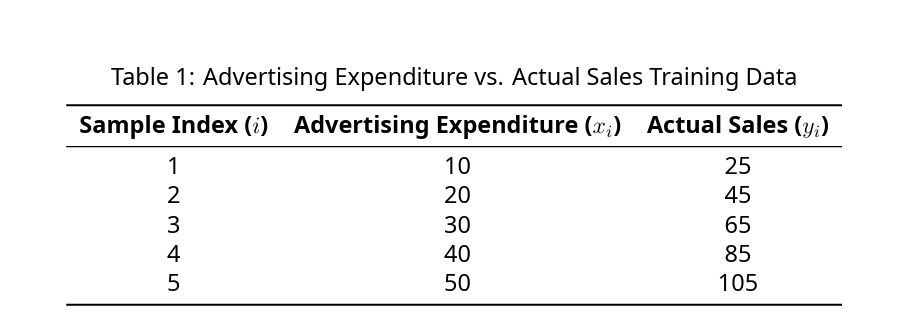
\includegraphics[width=7.65in,height=2.10in,keepaspectratio]{assets/p10_1.png}\end{center}
}

\sectionbar{9.10}{14.86}{8.35}{0.66}{Case study}
\card{9.10}{15.64}{8.35}{7.05}{%
\begin{center}
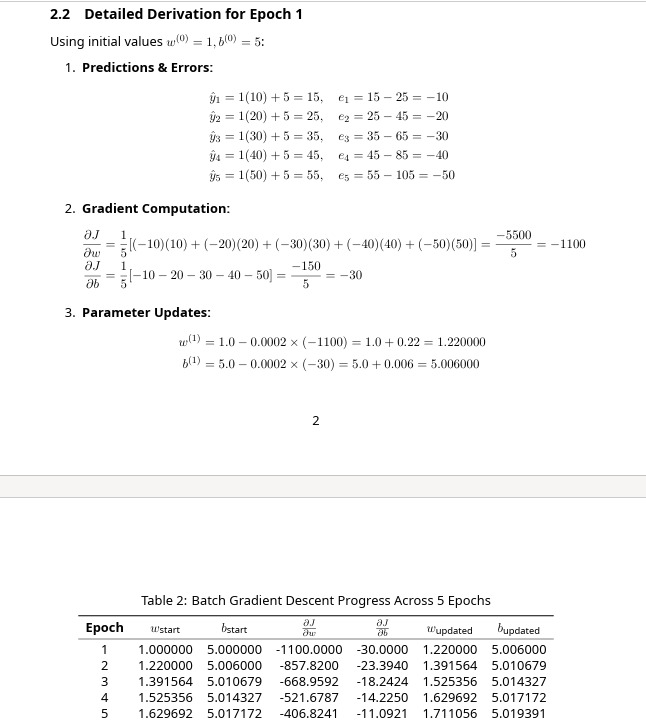
\includegraphics[width=3.89in,keepaspectratio]{assets/p11_1.png}\hspace{0.08in}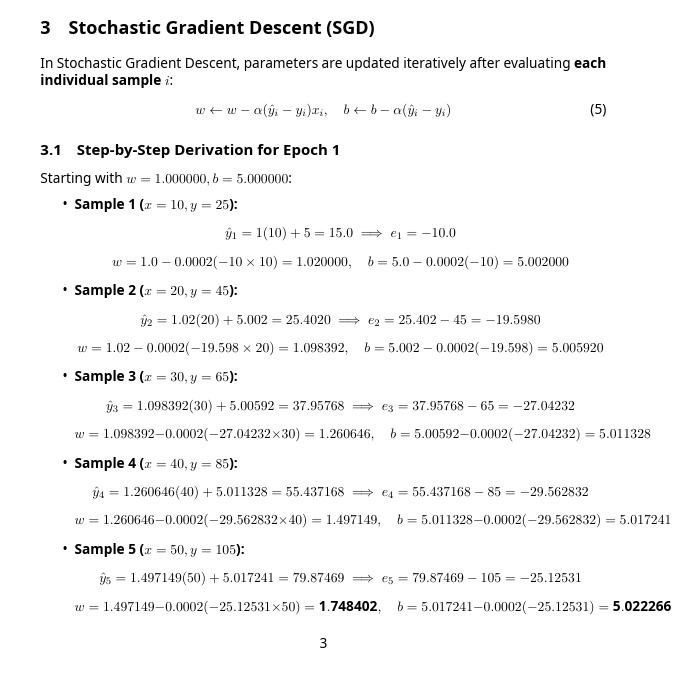
\includegraphics[width=3.89in,keepaspectratio]{assets/p11_2.png}
\end{center}
\vspace{2pt}
\sffamily\fontsize{13.7}{16.5}\selectfont\color{bodytext}\RaggedRight
The case study records parameter updates for Gradient Descent and Stochastic Gradient Descent. The source report uses the five-observation sales dataset and tracks $w$ and $b$ across training epochs.
}

\sectionbar{18.00}{14.86}{8.40}{0.66}{Comparison with Another Algorithm}
\card{18.00}{15.64}{8.40}{7.05}{%
\sffamily\fontsize{14.8}{17.5}\selectfont\color{bodytext}\RaggedRight
\textbf{GD vs SGD Loss Graph}\\[2pt]
\begin{center}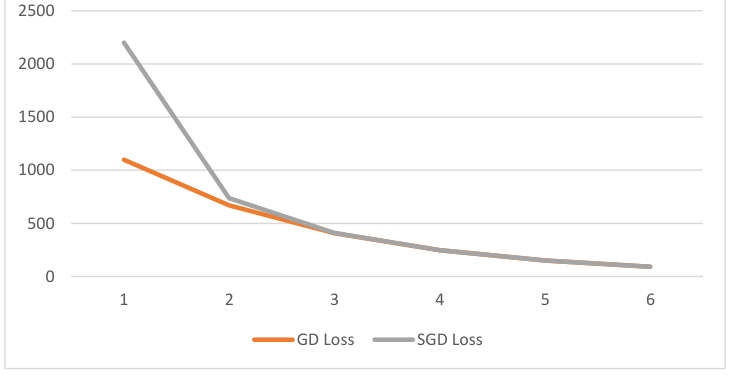
\includegraphics[width=7.55in,height=2.72in,keepaspectratio]{assets/loss_convergence_graph.png}\end{center}
\vspace{1pt}
\textbf{GD vs. SGD Loss Convergence}\\[2pt]
In this case study, the loss reduction of Gradient Descent (GD) and Stochastic Gradient Descent (SGD) is compared for six recorded epochs. The GD loss decreases from 1100 to 91.5017, while the SGD loss decreases from 1100 to 0.001. The graph shows the difference in loss reduction and convergence behavior between GD and SGD.
}

% References are intentionally adjacent to the comparison box.
\sectionbar{27.02}{14.86}{8.40}{0.66}{References}
\card{27.02}{15.64}{8.40}{7.05}{%
\sffamily\fontsize{11.6}{14.0}\selectfont\color{bodytext}\RaggedRight
\textbf{1. Gradient Descent intuition}\\[-1pt]
It explains the intuition behind Gradient Descent, optimization, and its application to Linear Regression.\\[-1pt]
\href{https://web.stanford.edu/class/cs168/l/gradDescNotes.pdf?utm_source=chatgpt.com}{Stanford CS168 — Gradient Descent Notes}\\[6pt]

\textbf{2. Gradient Descent in Linear Regression}\\[-1pt]
Linear Regression, MSE/Cost Function, Learning Rate, Gradient Calculation, Parameter Update, Iteration/Convergence.\\[-1pt]
\href{https://www.geeksforgeeks.org/machine-learning/gradient-descent-in-linear-regression/?utm_source=chatgpt.com}{GeeksforGeeks — Gradient Descent in Linear Regression}\\[6pt]

\textbf{3. Stochastic Gradient Descent (SGD)}\\[-1pt]
Single training example, parameter update, learning rate, gradient calculation, iterative process, faster updates, noisy/fluctuating updates.\\[-1pt]
\href{https://www.geeksforgeeks.org/ml-stochastic-gradient-descent-sgd/?utm_source=chatgpt.com}{GeeksforGeeks — Stochastic Gradient Descent (SGD)}\\[6pt]

\textbf{4. Book reference}\\[-1pt]
The concept of Gradient Descent is based on Nafis Neehal's \textit{Machine Learning Algorithms} (2018), p. 47.\\[-1pt]
Neehal, N. (2018). \textit{Machine Learning Algorithms}. 5th print, January 2022, p. 47.
}

\footer
\end{tikzpicture}
\end{document}
